Ray-casting the sphere is a trivial task; nevertheless, in our case the surface sphere of molecules might be formed by an arbitrary number of spherical patches lying in different surface components. To avoid obvious rendering issues, i.e., distinct coloring, transparency, or visibility, we perform ray-casting of each spherical patch separately.
This allows us to visually distinguish between different surface components.

Since the boundaries of a spherical patch are formed by small circle arcs, we apply an odd-even rule for polygons~\cite{shimrat1962algorithm} to test whether a point lies inside the patch. 
First we compute the intersection points, $P_{front}$ and $P_{back}$, of a given ray with the patch sphere.
Here we describe the point-patch test for point $P_{front}=P$ only, since the same test is applied to $P_{back}$.
Before we apply the odd-even rule, we choose a point $T$ lying outside the patch.
Then, we test line $TP$, the shortest path on a sphere, for an intersection with each of the arcs delimiting the patch.
The intersection of a line $TP$ with the small circle arc, given by points $AB$, is computed in two steps (Fig.~\ref{fig:outer-point} left):
\begin{enumerate}
  \item Intersections of the circles containing the line $TP$ and the arc $AB$, which can intersect in up to two points.
  \item Intersection points are tested whether they belong to both the segment $TP$ and the arc $AB$.
\end{enumerate}
Finally, if the sum of all intersections, i.e., for all the sides, is odd then the point lies inside the patch.

\begin{figure}[htp]
  \centering
  \begin{subfigure}[c]{0.52\columnwidth}
    \centering
    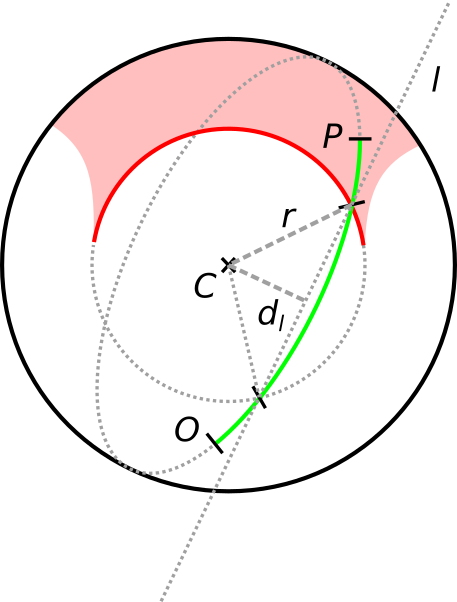
\includegraphics[height=1.9in]{image/patch.png}
    %\caption{%Point in spherical patch test.
		%The intersection $I_1$ lies on an intersection line between two planes containing arcs $OP$ and $AB$.}
		%\label{fig:spherical-patch}
  \end{subfigure}%
  \quad
  \begin{subfigure}[c]{0.44\columnwidth}
    \centering
    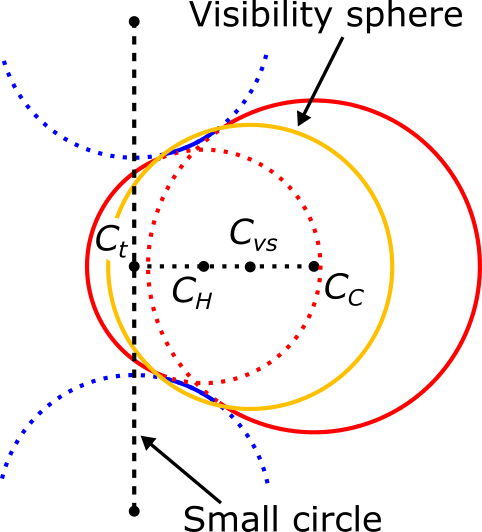
\includegraphics[height=1.6in]{image/outer.png}
    %\caption{%A torus formed by carbon ($C_C$) and hydrogen ($C_H$) atoms.
		%The center of the torus ($C_{t}$) lies outside the atom centers, while the center of its visibility sphere $C_{vs}$ lies between $C_C$ and $C_H$.}
  \end{subfigure}
\caption{Left: A point against the spherical patch test. The intersection $I_1$ lies on an intersection line between two planes containing arcs $OP$ and $AB$. Right: A torus formed by carbon ($C_C$) and hydrogen ($C_H$) atoms. The center of the torus ($C_{t}$) lies outside the atom centers, while the center of its visibility sphere $C_{vs}$ lies between $C_C$ and $C_H$.}
\label{fig:outer-point}
\end{figure}

Since we deal with spherical patches and not the planar ones, the situation is bit more complex and we cannot choose point $T$ arbitrarily. 
%Otherwise, we would count intersections of patch's sides with a great circle containing $P$.
%Then, the intersection count would be the same regardless of $P$ being inside or outside the patch, making the rule inapplicable.
Instead, we compute $T$ by intersecting a patch sphere by an axis of one of its delimiting tori.
In this way, we get two intersection points from which we choose the one that lies in the direction of the torus visibility sphere (Fig.~\ref{fig:outer-point} right).